\setcounter{chapter}{-1}
\chapter{Introduction: Fuzzy Logic as a Framework for Uncertainty in Decision Making}


Before stating a proper formalization of the fuzzy framework, it is crucial to first clarify what it represents and why there is a need for such a theory when there already exists Probability and Statistics, which are broadly applied and much more developed.\\

The main objective of these frameworks is to represent and manage uncertainty inherent in complex systems. This involves encoding data and expressing information through appropriate mathematical structures and developing measures that enable effective synthesis and combination of uncertain information.\\

A fundamental motivation for modeling uncertainty is to enable better decision making across diverse domains. In engineering, uncertainty quantification helps assess structural reliability and optimize designs. In finance, it aids risk management and portfolio optimization. In medicine, it supports diagnosis and treatment planning under incomplete information. In environmental science, it helps model climate patterns and ecological systems. By developing mathematical frameworks to represent and reason about uncertainty, we can make more informed choices and balance competing objectives in complex scenarios.\\

\section{Uncertainty: Definition and Types}

There is no consensus about a unique definition of uncertainty and a single classification of its types. 

As mentioned above, uncertainty is present in complex systems. According to \cite{UncertaintySciences}, \textbf{systems are abstractions that aid understanding} a group of interacting, interrelated, or interdependent elements that together form a complex whole, which can be a physical structure, process, or procedure with some attributes of interest. All parts of a system are related to the same overall process, procedure, or structure. \\

Notice that usually these abstractions are not unique in the sense that there are different ways to model the same system. Formally it is:

\begin{definition}[System]
    An object is called a system if it can be expressed as a pair of a set of things ($T$) and a set of relations ($R$).

    \[S = (T,R)\]
\end{definition}

\begin{remark}
    By \emph{set of things}, we mean that \(T\) may be any collection of elements, from a simple set (finite or infinite) to more complex structures such as sets of sets or power sets. Likewise, the \emph{set of relations} (\(R\)) is understood broadly, it encapsulates interactions, constraints, and dependencies between these elements; providing a structural foundation. Hence, even though \((T, R)\) appears simple, its components can be very varied and rich.
\end{remark}

This definition is too general to have any practical utility. However, it gives us a flexible "skeleton" to build upon and tackle what we refer to with \textit{uncertainty in a system}. \\

Finding a proper definition for uncertainty is a very subtle and challenging task due to the ample scope of the concept, but following the ideas from \cite{UncertaintySciences} and \cite{RumsfeldMatrix} we will start by classifying knowledge into 4 categories using Rumsfeld's Matrix\footnote{While \cite{RumsfeldMatrix} classifies this matrix as representing only Epistemic Uncertainty, we take a broader view since aleatoric uncertainty, with its quantifiable regularities through probability distributions, can be considered a "known unknown".}:

\begin{table}[h!]
    \centering
    \label{tab:rumsfeld}
    \begin{tabular}{@{}c@{~}c|c|c|}
        \multicolumn{2}{c}{} & \multicolumn{2}{c}{\large \textbf{Our Perceived Knowledge}} \\[0.3em]
        \multicolumn{2}{c}{} & \multicolumn{1}{c}{Known} & \multicolumn{1}{c}{Unknown} \\
        \cline{3-4}
        \multirow{2}{*}{\rotatebox{90}{\parbox{2cm}{\centering \large \textbf{Real State of} \\ \textbf{Knowledge}}}} 
        & Known & Things we know we know & Things we know we don't know \\
        \cline{3-4}
        & Unknown & Things we know we don't know & Things we do not know we don't know \\
        \cline{3-4}
    \end{tabular}
    \vspace{1cm}
    \caption{Rumsfeld's Matrix}
\end{table}

This matrix illustrates the relationship between knowledge and ignorance\footnote{For a more rigorous treatment of ignorance and higher-order ignorance using non-formal modal logic see \cite{firstorderignorance}.}, where ignorance can be understood as the absence or incompleteness of knowledge. In particular, we would consider \textbf{ignorance} to be represented in the \textit{Unknown} column and \textbf{knowledge}, in the \textit{Known} column. From this perspective, we can identify:
% \begin{itemize}
%     \item \textbf{Known Knowns}: things we are aware of and understand well.
%     \item \textbf{Unknown Knowns}: these are the aspects that we actually know but are not conciously aware of. They might include tacit knowledge or assumptions that go unrecognized.
%     \item \textbf{Known Unknowns}: gaps in our knowledge that we recognize.
%     \item \textbf{Unknown Unknowns}: things we are completely unaware of.
% \end{itemize}
 
\begin{tikzpicture}[remember picture, every node/.style={anchor=west}]
    % First group: Knowledge
    \node (knowledge) at (0,0) {%
      \begin{minipage}{0.8\textwidth}
        \begin{itemize}[leftmargin=1cm]
          \item \textbf{Known Knowns}: things we are aware of and understand well.
          \item \textbf{Unknown Knowns}: these are the aspects that we actually know but are not consciously aware of.
        \end{itemize}
      \end{minipage}%
    };
    
    % Second group: Ignorance
    % Increase vertical gap below "knowledge" to avoid overlap
    \node (ignorance) [below=0.5cm of knowledge] {%
      \begin{minipage}{0.8\textwidth}
        \begin{itemize}[leftmargin=1cm]
          \item \textbf{Known Unknowns}: gaps in our knowledge that we recognize.
          \item \textbf{Unknown Unknowns}: things we are completely unaware of.
        \end{itemize}
      \end{minipage}%
    };
    
    % Draw curly brace for Knowledge
    % Shift it further left (xshift=-1.2cm) and move label out (xshift=-0.6cm)
    \draw[
      decorate,
      decoration={brace, amplitude=10pt, mirror}
    ] 
      ([xshift=0.6cm]knowledge.north west) 
      -- 
      ([xshift=0.6cm]knowledge.south west)
      node[midway, left, xshift=-0.6cm,yshift=1cm, rotate=90] {\large Knowledge};
    
    % Draw curly brace for Ignorance
    \draw[
      decorate,
      decoration={brace, amplitude=10pt, mirror}
    ] 
      ([xshift=0.6cm]ignorance.north west) 
      -- 
      ([xshift=0.6cm]ignorance.south west)
      node[midway, left, xshift=-0.6cm,yshift=1cm, rotate=90] {\large Ignorance};
  \end{tikzpicture}

In the context of uncertainty quantification, we focus primarily on the \textbf{known unknowns} because those are the aspects of ignorance that we can identify and attempt to model. Therefore, we can finally state what we will consider as uncertainty in this work:\\


\begin{definition}[Uncertainty in a system]
    \say{The term uncertainty can be viewed as \textbf{a component of ignorance}.[...] Uncertainty and information as a pair, and ignorance and knowledge as another pair,[...], as the former component of each pair describes a deficiency in the respective latter component, while the latter component of a pair can be viewed as the respective capacity available to reduce the respective former component.}\cite{UncertaintySciences}
\end{definition}

It is useful to classify different types of uncertainty to better understand what our mathematical models represent. However, it is vital to keep in mind that these types are not independent of each other. Rather than strict boundaries where every known unknown fits, it is better to think of them as dimensions of uncertainty. The most broadly used classification of uncertainty is this binary one:\\

\begin{itemize}
    \item \textbf{Aleatoric:} inherent randomness or natural variability, which is \textbf{irreducible}. This is the most familiar one to the general public since it is the one that appears in the famous example of throwing a fair dice, and it is a case of success of probability theory.
    \item \textbf{Epistemic Uncertainty}: arises from incomplete knowledge, measurement limitations, imperfect models, or lack of data. This uncertainty \textbf{may be reducible} if additional information or resources become available. Some examples include: 
    \begin{itemize} 
        \item Estimating voter preferences from a poll of 10 people involves high epistemic uncertainty; polling 10,000 voters significantly reduces this uncertainty, providing a clearer representation of true preferences. 
        \item Imagine a sensor that detects if a temperature is above a threshold. Even if we have 2 objects at different temperature above that level, we would need to group them together. This situation presents uncertainty due to the limited granularity of our knowledge, known as \textbf{coarseness} (which is a type of epistemic uncertainty).
    \end{itemize} 
\end{itemize}

Nevertheless, this binary classification has several important limitations:

\begin{itemize}
    \item \textbf{Incomplete Coverage:} Some forms of uncertainty do not neatly fit into these two categories. For example: vagueness, which is not aleatoric but neither reducible with more data.
    \item \textbf{Fail to capture higher-order uncertainties:} does not account for meta-uncertainties (uncertainty about the uncertainty itself) or a broader hierarchical nature of ignorance.
    \item \textbf{Interdependence Oversight:} The influence between each other is not taken into account.
\end{itemize}

A classification of uncertainty types allow us to build a proper representation tailored to a specific kind of ignorance. Given these limitations of the binary classification, we will adopt a more nuanced framework based on \cite{UncertaintySciences}. While their full classification system is more extensive than needed for our purposes, we will present a simplified version that better captures the complexity of uncertainty while remaining practical for our analysis. It is important to note that while specific frameworks are associated with each type of uncertainty (even the same framework with multiple uncertainty types), alternative modeling approaches exist and can be effectively used.


\begin{itemize}
    \item \textbf{Nonspecificity:} Uncertainty resulting from insufficient specificity or detail, information is insufficient to precisely specify which outcome or event applies.
    \begin{itemize}
        \item \textit{Example:} Knowing only that the solution to an equation lies within a set \(\{1, 2, 3\}\), but without further precision.
        \item \textit{Frameworks:} Modeled primarily by crisp set theory and possibility theory, where uncertainty arises from ambiguous specification of possibilities.
    \end{itemize}

    \item \textbf{Vagueness:} Arises from imprecise, unclear, or fuzzy boundaries in concepts, meaning that elements can partially belong to a category. 
    \begin{itemize}
        \item \textit{Example:} Categorizing a temperature as "hot"; the boundary between hot and not-hot is not clearly defined; it is not crisp.
        \item \textit{Frameworks:} Modeled using fuzzy set theory, assigning partial membership values between 0 and 1 to indicate degrees of compatibility between elements and sets.
    \end{itemize}

    \item \textbf{Coarseness (Granularity):} Uncertainty due to limited resolution in the available data or knowledge, making it difficult to distinguish precisely between similar elements.
    \begin{itemize}
        \item \textit{Example:} A doctor has patient records with temperatures and cough symptoms, but can only match new patients' temperatures with cough symptoms at a coarse level (e.g. 37.3°C and 37.4°C are treated as identical since the records don't include every possible temperature value), limiting the precision of symptom prediction.
        \item \textit{Frameworks:} Modeled using rough set theory, i.e. equivalence classes to define lower and upper approximations of a set to manage indistinguishability caused by granularity.
    \end{itemize}

    \item \textbf{Randomness (Aleatoric Uncertainty):} Intrinsic uncertainty in stochastic processes, inherently irreducible, even with complete knowledge of the system.
    \begin{itemize}
        \item \textit{Example:} Predicting the outcome of a fair dice roll.
        \item \textit{Frameworks:} Modeled by probability theory through probability distributions, which represent expected frequencies in repeated experiments but unable to deterministically predict individual outcomes.
    \end{itemize}

    \item \textbf{Epistemic Uncertainty:} Uncertainty arising from incomplete understanding of the true structure, parameters, or mechanisms governing a system. This can include potentially missing or incorrect model assumptions. It is often considered reducible through targeted investigations, refining model assumptions, or incorporating more informative data expanding the knowledge of the underlying system.

    \begin{itemize}
        \item \textit{Example:} Modeling a physical process but without knowing whether it is linear or nonlinear; further experiments could reveal the correct functional form.
        \item \textit{Frameworks:} Often modeled via Bayesian inference (updating priors with data), possibility theory, belief functions, and interval methods. The focus is on refining or correcting a model (e.g., identifying correct distributions, dependencies, causal structures).
    \end{itemize}

    \item \textbf{Sampling Uncertainty:} Uncertainty emerging from inferring properties of a population based solely on a limited sample from it.
    \begin{itemize}
        \item \textit{Example:} Estimating the average height of a country's population from measurements of a random subset.
        \item \textit{Frameworks:} Modeled by inferential statistics, confidence intervals, hypothesis testing, and conformal prediction methods, explicitly quantifying the variability and uncertainty in such inferences.
    \end{itemize}
\end{itemize}

A final consideration worth discussing is \textbf{the distinction between subjectivity and objectivity in uncertainty representation}. 
This distinction plays an important role in frameworks like Bayesian statistics (through the specification of prior distributions) and is particularly relevant in fuzzy set theory where membership values often reflect a decision maker's subjective assessment. However, while the source of uncertainty may differ (subjective judgment versus objective measurement), we will treat them as formally equivalent in their mathematical representation. The only practical distinction may arise when decision makers assign importance weights, potentially weighting objective and subjective sources differently according to their preferences.\\

The boundary between what may be considered objective versus subjective in fuzzy sets is often unclear. Consider this illustrative example that highlights this ambiguity:
Suppose we want to determine the membership degree of a person who is 180cm tall to the set of "tall people". One approach would be to assign a value based on personal perception, a subjective assessment influenced by our own height, the heights of people we know, and even potentially varying over time as our perception changes. Alternatively, we could use the population height percentile as the membership degree, which seems more objective. However, this choice still involves subjective decisions: for instance, why use the percentile directly rather than its square root?\\

Therefore, throughout this work, we will treat subjective and objective uncertainties as formally equivalent, with the only potential distinction arising from how decision makers may choose to weight their relative importance in specific contexts.

\section{Vagueness and Sorites Paradox}

Among the uncertainty types discussed above, vagueness is most relevant to the following chapters, as it is mainly modeled using fuzzy sets.\\

Fuzzy sets extend classical (or crisp) sets by introducing partial memberships, moving beyond the binary notion of "belongs" or "doesn't belong". This provides a more expressive framework for modeling concepts that cannot be adequately represented using traditional sets.\\

To demonstrate the necessity of fuzzy sets and following \cite{HájekSorites}, let us consider the Sorites Paradox. Attributed to the philosopher Eubulides, this paradox emerges from the following type of reasoning:

\begin{enumerate}
    \item A single grain of sand does not form a heap.
    \item Adding one grain to something that is not a heap does not make it a heap.
    \item Consequently, there are no heaps.
\end{enumerate}


There are many variations of this paradox with different vague concepts such as age, size, height, baldness, etc. All share the same issue: there is a gradual transition, and evaluating to only true or false does not allow us to represent it adequately, therefore reaching a contradiction.\\

This paradox can be resolved by considering partial membership to the set of heaps, where a single grain may have 0.001 membership which grows with the number of grains until reaching a group of a million grains, which could have 1 membership. While these numbers are arbitrary, this model better captures our intuitive concept of a heap than the conclusion that "heaps don't exist".\\

However, in the paradox we are dealing with truth values rather than membership. In this case, the concepts are completely analogous, as there is a direct relationship between the membership degree of an amount of grains to the set of heaps and the truth value of the proposition \textit{"This amount of grains is a heap"}. In the paper \cite{HájekSorites}, the authors argue that the proposition "\textit{Adding one grain to something that is not a heap does not make it a heap}" is not strictly true but rather almost true, thus by considering varying degrees of truth we avoid the contradiction.\\

This example illustrates how vagueness is the core issue with these concepts: the boundary of the set of heaps is not crisp but rather fuzzy. There is no precise point where something transitions from not being a heap to being one, it is a gradual process. \\

In the following chapters, we will demonstrate that fuzzy logic and the treatment of vagueness is not merely an academic curiosity, but rather a powerful framework with both practical applications and rigorous theoretical foundations. 

\section{Mathematical Uncertainty Theories}

As mentioned in \cite{uncertaintymeasuresbigpicture} and further detailed in chapters 2 and 3 of \cite{UncertaintySciences}, a theory of uncertainty typically consists of two elements:

\begin{romanenum}
    \item A mathematical representation that encodes data about uncertain states of the world.
    \item Mathematical operators and measures that enable reasoning about and combining uncertain information.
\end{romanenum}

As shown in Figure \ref{fig:Generalized_sets}, data is encoded via different types of sets, according to what is considered precise or not (elements and sets). These set models are examples of theories that tackle a specific representation, but are not the only possible models.\\

When choosing a proper model for a concrete problem, one should 
take into account that the more expressive and general a framework 
is, the more complicated it becomes due to all the nuances it 
attempts to capture. For this reason, \textbf{precise information should be modeled as precise rather than imprecise when available}. This trade-off will be explored further in the discussion of possibilities and probabilities, where possibilities offer greater expressiveness but lower predictive power.


\begin{figure}[ht]
    \hspace{2cm}
    \begin{tikzpicture}[>=stealth, font=\sffamily, align=center]
        % Define column x-positions.
        \def\xOne{-3}   % Column 1: Elements of Universal Set
        \def\xTwo{0}    % Column 2: Set (or event as a notion)
        \def\xThree{3}  % Column 3: Set Membership
        \def\xFour{6}   % Column 4: Example Theories
        
        % Use a common vertical center (here chosen as 0).
        \def\Bgap{0.75}
        
        % Column 2 vertical shifts.
        \def\CshiftA{2.25}
        \def\CshiftB{0.75}
        \def\CshiftC{-0.75}
        \def\CshiftD{-2.25}
        
        % Column 3 and Column 4 vertical shifts.
        \def\Dshiftone{5.25}
        \def\Dshifttwo{3.75}
        \def\Dshiftthree{2.25}
        \def\Dshiftfour{0.75}
        \def\Dshiftfive{-0.75}
        \def\Dshiftsix{-2.25}
        \def\Dshiftseven{-3.75}
        \def\Dshifteight{-5.25}
        
        % --------------------- Column 1 ---------------------
        % Small nodes
        \node (B1) at (\xOne, \Bgap)
              [rectangle, draw, fill=blue!10] {Precise\\ elements};
        \node (B2) at (\xOne, -\Bgap)
              [rectangle, draw, fill=blue!10] {Imprecise\\ elements};
              
        % Big rectangle in the background layer
        \begin{pgfonlayer}{background}
        \node[draw, thick, rounded corners,
              fill=gray!10,
              fit=(B1)(B2),
              inner sep=5pt,
              label={[align=center]above:\textbf{Elements}}
        ] (BoxB) {};
        \end{pgfonlayer}
        
        % --------------------- Column 2 ---------------------
        \node (C1) at (\xTwo, \CshiftA)
              [rectangle, draw, fill=blue!10] {Precise\\ set};
        \node (C2) at (\xTwo, \CshiftB)
              [rectangle, draw, fill=blue!10] {Imprecise\\ set};
        \node (C3) at (\xTwo, \CshiftC)
              [rectangle, draw, fill=blue!10] {Precise\\ set};
        \node (C4) at (\xTwo, \CshiftD)
              [rectangle, draw, fill=blue!10] {Imprecise\\ set};
        
        \begin{pgfonlayer}{background}
        \node[draw, thick, rounded corners,
              fill=gray!10,
              fit=(C1)(C4),
              inner sep=5pt,
              label={[align=center]above:\textbf{Set}}
        ] (BoxC) {};
        \end{pgfonlayer}
        
        % --------------------- Column 3 ---------------------
        \node (D1) at (\xThree, \Dshiftone)
              [rectangle, draw, fill=blue!10] {Binary};
        \node (D2) at (\xThree, \Dshifttwo)
              [rectangle, draw, fill=blue!10] {Non-\\binary};
        \node (D3) at (\xThree, \Dshiftthree)
              [rectangle, draw, fill=blue!10] {Binary};
        \node (D4) at (\xThree, \Dshiftfour)
              [rectangle, draw, fill=blue!10] {Non-\\binary};
        \node (D5) at (\xThree, \Dshiftfive)
              [rectangle, draw, fill=blue!10] {Binary};
        \node (D6) at (\xThree, \Dshiftsix)
              [rectangle, draw, fill=blue!10] {Non-\\binary};
        \node (D7) at (\xThree, \Dshiftseven)
              [rectangle, draw, fill=blue!10] {Binary};
        \node (D8) at (\xThree, \Dshifteight)
              [rectangle, draw, fill=blue!10] {Non-\\binary};
        
        \begin{pgfonlayer}{background}
        \node[draw, thick, rounded corners,
              fill=gray!10,
              fit=(D1)(D8),
              inner sep=5pt,
              label={[align=center]above:\textbf{Set Membership}}
        ] (BoxD) {};
        \end{pgfonlayer}
        
        % --------------------- Column 4 ---------------------
        \node (E1) at (\xFour, \Dshiftone)
              [rectangle, draw, fill=blue!10] {Crisp\\ sets};
        \node (E2) at (\xFour, \Dshifttwo)
              [rectangle, draw, fill=blue!10] {Rough\\ sets};
        \node (E3) at (\xFour, \Dshiftthree)
              [rectangle, draw, fill=blue!10] {Illogical};
        \node (E4) at (\xFour, \Dshiftfour)
              [rectangle, draw, fill=blue!10] {Fuzzy\\ sets};
        \node (E5) at (\xFour, \Dshiftfive)
              [rectangle, draw, fill=blue!10] {Illogical};
        \node (E6) at (\xFour, \Dshiftsix)
              [rectangle, draw, fill=blue!10] {Fuzzy\\ rough sets};
        \node (E7) at (\xFour, \Dshiftseven)
              [rectangle, draw, fill=blue!10] {Illogical};
        \node (E8) at (\xFour, \Dshifteight)
              [rectangle, draw, fill=blue!10] {Rough\\ fuzzy sets};
        
        \begin{pgfonlayer}{background}
        \node[draw, thick, rounded corners,
              fill=gray!10,
              fit=(E1)(E8),
              inner sep=5pt,
              label={[align=center]above:\textbf{Set Models}}
        ] (BoxE) {};
        \end{pgfonlayer}
        
        % --------------------- Edges ---------------------
        % Column 1 -> Column 2:
        \draw[->] (B1) to[bend right=10] (C1);
        \draw[->] (B1) to[bend left=10] (C2);
        \draw[->] (B2) to[bend right=10] (C3);
        \draw[->] (B2) to[bend left=10] (C4);
        
        % Column 2 -> Column 3:
        \draw[->] (C1) to[bend right=10] (D1);
        \draw[->] (C1) to[bend left=10] (D2);
        \draw[->] (C2) to[bend right=10] (D3);
        \draw[->] (C2) to[bend left=10] (D4);
        \draw[->] (C3) to[bend right=10] (D5);
        \draw[->] (C3) to[bend left=10] (D6);
        \draw[->] (C4) to[bend right=10] (D7);
        \draw[->] (C4) to[bend left=10] (D8);
        
        % Column 3 -> Column 4:
        \draw[->] (D1) -- (E1);
        \draw[->] (D2) -- (E2);
        \draw[->] (D3) -- (E3);
        \draw[->] (D4) -- (E4);
        \draw[->] (D5) -- (E5);
        \draw[->] (D6) -- (E6);
        \draw[->] (D7) -- (E7);
        \draw[->] (D8) -- (E8);
        
    \end{tikzpicture}
    \caption{Generalizations of crisp sets with different set models, showing increasing levels of expressivity for encoding data uncertainty. Adapted from Figure 2.1 in \cite{UncertaintySciences}.}
    \label{fig:Generalized_sets}
\end{figure}



Regarding operators and measures (most based on the previous set models), there exist many different frameworks, with varying levels of development and adoption. In Figure \ref{fig:uncertainty_taxonomy}, Cuzzolin \cite{uncertaintymeasuresbigpicture} maps out the major uncertainty theories and notes that \say{The \say{quality} of the various proposals differs radically}. As an example, he points out that Liu's Uncertainty Theory lacks rigorous mathematical foundations and convincing justification. \\

Another interesting observation stated in the paper is that generality isn't the only factor that matters, as the most general frameworks haven't experienced the growth and adoption one might expect. This is likely because overly general frameworks can become intractable and unnecessarily complex without providing clear practical benefits:

\hspace{1cm}\say{Imprecise probability is remarkable for its generality, as special cases of coherent lower previsions include probabilities, de Finetti previsions, Choquet capacities, possibility and belief measures, random sets but also probability boxes, (lower and upper envelopes of) credal sets, and robust Bayesian models. Nevertheless, IP has so far failed to achieve the expected impact in both mathematical statistics and application fields. This may lead to the reflection that generality, after all, is not the real thing.}\cite{uncertaintymeasuresbigpicture}\\

The majority of these frameworks emerged to address key limitations of probability theory. Some of these limitations include:
\begin{romanenum}
      \item \textbf{Second-Order Uncertainty:} Probability theory handles risk well but fails to capture uncertainties about the probability model itself.
      \item \textbf{Ignorance Representation:} There is no probability distribution that assigns equal probability to every single event (not even the uniform distribution). There the state of absolute ignorance is not possible.
      \item \textbf{Imprecision in Data:} The additive nature of probability struggles with fuzzy, ambiguous, or set-valued data.
      %\item \textbf{Scarce Data Limitations:} It relies on large datasets, making it less effective when data is incomplete or limited.
      \item \textbf{Additivity Constraint:} The strict additivity axiom prevents modeling non-additive phenomena common in real-world uncertainty.
      %\item \textbf{Update and Combination Challenges:} Bayesian inference requires well-justified priors and often struggles to combine uncertain evidence.
      %\item \textbf{Alternative Reasoning Incompatibility:} It does not integrate smoothly with frameworks like fuzzy logic or belief functions.
      %\item \textbf{Decision-Making Mismatch:} Observed human behavior under uncertainty (e.g., Ellsberg's paradox) often contradicts classical probabilistic predictions.
      \item \textbf{Rigidity in Assumptions:} The need for well-defined sample spaces and distributions is frequently unrealistic in complex, real-world scenarios.
    \end{romanenum}
    




\begin{figure}[ht]
    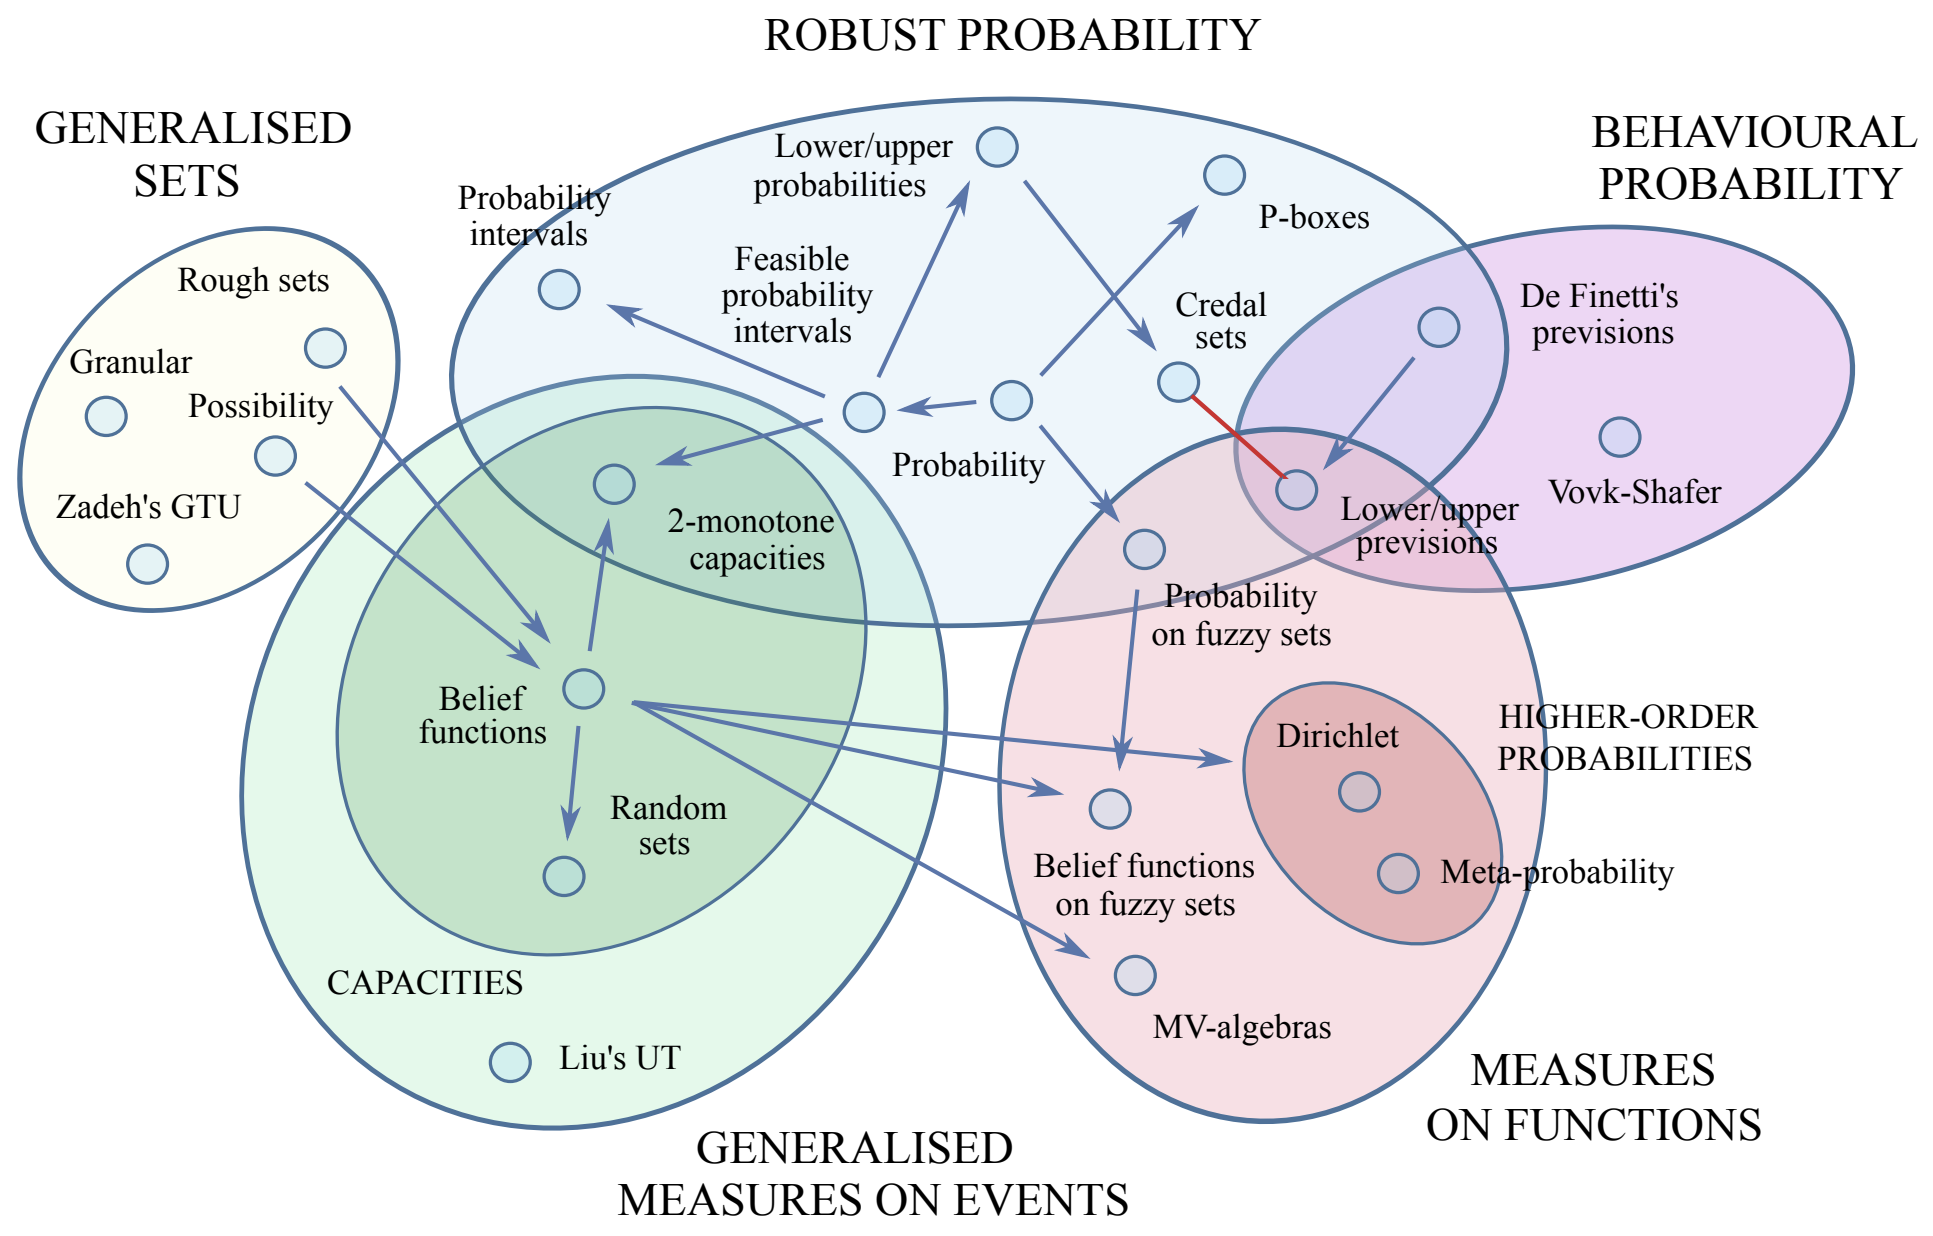
\includegraphics[width=\textwidth]{ch0/figures/Uncertainties Diagram.png}
    \caption{A classification of uncertainty theories showing their relationships and hierarchies. The theories are grouped based on their rationale and class of objects they attempt to mathematically model. Arrows indicate generalization relationships, pointing from more specific to more general frameworks. Extracted from \cite{uncertaintymeasuresbigpicture}.}
    \label{fig:uncertainty_taxonomy}
\end{figure}













































\section{Structure of this work}


\signal{What are the different kinds of uncertainty, why not simply use probability for modeling uncertainty, the sorites paradox, what are rough sets (very briefly like in a couple of paragraphs to outline) and what is the structure of this book.

I don't want to state any definitions and things, that is inside the main work and other chapters where those are properly stated.


}



\signal{Pongo mi propia clasificacion:
aleatoric (probabilidad), epistemic (falta de datos únicamente) eso tiene que ver con cómo de bueno es el modelo, pero no tenemos un framework específico creo. Luego van vagueness (fuzzy) y coarseness (rough).

Creo que voy a tener que mencionar lo de subjetividad y objetividad, que aquí no vamos a hacer distinción ya que formalmente son iguales, aunque se las trate de maneras diferentes. Una distribución es una distribución a nivel formal. No vamos a tratarlo de forma diferente salvo quizás por lo relevante que el decision maker lo considere. 

En Vagueness explico la paradoja de sorites

Luego explico lo que es la representación de la data y lo otro:
A theory of uncertainty is typically composed of two elements: (i) a mathematical object encoding an uncertain state 
of the world, and (ii) an operator which allows us to reason
with uncertain states

Hablo también de que hay muchísimos modelos, de que cuantificar incertidumbre es ponerle vayas al campo y de cómo es relevante encontrar un equilibrio entre modelizar todos los detalles y que sea práctico y se pueda trabajar con algo que no es absurdamente complejo.

Finalmente presento los capítulos (el de possibility distributions, lo saco del primer capítulo mejor)}






